\section{Trig (II): Graphs and Inverses}

\subsection{Review problems}

\begin{enumerate}
\item \emph{The six basic graphs.} Match each of the graphs below to one of the six basic trig functions.
\begin{figure}[H]
\centering
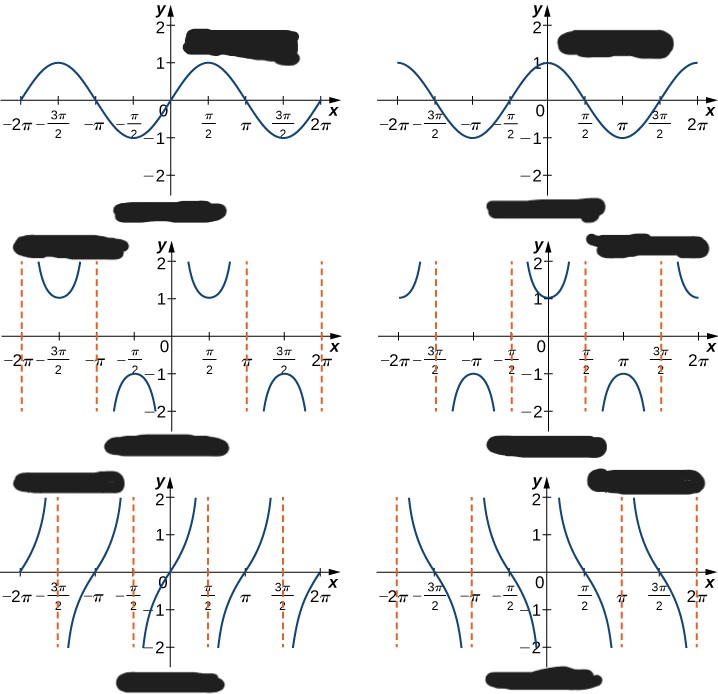
\includegraphics[scale=0.7]{img-trig-graphs.jpg}
\end{figure}
\item \emph{Period and frequency.} A function $f:\mathbb{R}\to\mathbb{R}$ is \emph{periodic} if there is a non-zero real number $T$ such that $f(x + T) = f(x)$ for all real $x$. Any such $T$ is a \emph{period} of $f$, and the smallest such positive $T$, if it exists, is the \emph{fundamental period} of $f$. If $f$ is a periodic function with fundamental period $T$, the \emph{natural frequency} of $f$ is $\nu = 1/T$ while the \emph{angular frequency} of $f$ is $\omega = 2\pi/T = 2\pi\nu$. Usually, ``the period'' of a periodic function means its fundamental period, while ``a period'' can be any period (not just the fundamental period). For each of the six basic trig functions, what are the period, natural frequency, and angular frequency?
\item \emph{Transformed sinusoidal waves.} For each of the following functions $\mathbb{R}\to\mathbb{R}$, find the period, amplitude, and phase shift relative to $\sin(\omega x)$, where $\omega$ is the angular frequency of the function.
\begin{enumerate}
\item $\sin x$
\item $\cos x$
\item $3\sin(5x - \tfrac{\pi}{7})$
\item $2\sin(2x) - 2\cos(2x)$
\end{enumerate}
\item \emph{Domain and range.} What are the standard domains and ranges of $\arcsin$, $\arccos$, and $\arctan$?\newpage
\item \emph{Calculating inverses.}
\begin{enumerate}
\item $\arcsin(1/2)$
\item $\arccos\left(-1/\sqrt{2}\right)$
\item $\arcsin\left(-\sqrt{3}/2\right)$
\item $\arctan(-1)$
\item $\arcsin(\sin(7\pi/6))$
\item $\cos(\arccos(-1/3))$
\item $\cos(\arctan(1/2))$
\end{enumerate}
\item \emph{Counting solutions.} Find the number of solutions for $x$ in each of the following equations.
\begin{enumerate}
\item $\sin\theta = 0.5$ when $0\leq\theta < 2\pi$
\item $\cos\theta = -2$ when $0\leq\theta < 2\pi$
\item $\sec\theta = 1$ when $-\pi < \theta\leq\pi$
\item $\tan\theta = 1$ when $-\pi < \theta\leq\pi$
\item $\sin(3\theta) = 0.2024$ when $0\leq\theta < 10\pi$
\item $\cos(\frac{22}{7}\theta) = 0.5$ when $-20 < \theta < 20$
\end{enumerate}
\item What are the standard domains and ranges of $\sec^{-1}$, $\csc^{-1}$, and $\cot^{-1}$?
\end{enumerate}


\subsection{Challenge problems}

\begin{enumerate}\setcounter{enumi}{7}
\item Karen has a calculator which only has seven buttons: $\sin$, $\cos$, $\tan$, $\arcsin$, $\arccos$, $\arctan$, and Reset. The first six apply these functions to the number in the display, while Reset changes the display back to its default state of showing 0. All calculations assume radian measure.
\begin{enumerate}
\item Starting from a positive real number $x$ in the display, show that there is a sequence of buttons that changes the display to $1/x$.
\item Starting from a non-negative real number $x$ in the display, show that there is a sequence of buttons that changes the display to $\sqrt{x^2 + 1}$.
\item Show that for every positive rational number $q$, there is a sequence of buttons that changes the display from $0$ to $\sqrt{q}$.
\end{enumerate}
\item Find the period of the following functions, or show that no period exists.
\begin{enumerate}
\item $\sin(3x) + \sin(4x)$
\item $\sin(20x) + \sin(24x)$
\item $\sin(x) + \sin(\sqrt{2}x)$
\end{enumerate}
\item A function $f:\mathbb{C}\to\mathbb{C}$ is \emph{doubly-periodic} if there are non-zero constants $u,v\in\mathbb{C}$ such that $u/v$ is non-real and $f(z) = f(z + u) = f(z + v)$ for all complex numbers $z$. Write down an example of a non-constant doubly-periodic function.
\end{enumerate}


\newpage
\subsection{Answers}

\begin{enumerate}
\item top left is sine; top right is cosine;\par
middle left is cosecant; middle right is secant;\par
bottom left is tangent; bottom right is cotangent
\item sine, cosine, secant, cosecant have period $2\pi$, natural frequency $\frac{1}{2\pi}$, angular frequency 1;\par 
theirangent, cotangent have period $\pi$, natural frequency $\frac{1}{\pi}$, angular frequency 2
\item \begin{enumerate}
\item period $2\pi$; amplitude $1$; phase shift $0$
\item period $2\pi$; amplitude $1$; phase shift $-\pi/2$ since $\cos x = \sin\left(x + \frac{\pi}{2}\right)$
\item period $2\pi/5$; amplitude $3$; phase shift $\pi/35$
\item period $\pi$; amplitude $2\sqrt{2}$ since $2\sin(2x) - 2\cos(2x) = 2\sqrt{2}\sin\left(2x - \frac{\pi}{4}\right)$; phase shift $\pi/8$
\end{enumerate}
\item arcsin has domain $[-1,1]$ and range $[-\pi/2, \pi/2]$;\par
arccos has domain $[-1,1]$ and range $[0,\pi]$;\par
arctan has domain $\mathbb{R}$ and range $(-\pi/2, \pi/2)$
\item \begin{enumerate}
\item $\pi/6$
\item $3\pi/4$
\item $-\pi/3$
\item $-\pi/4$
\item $-\pi/6$
\item $-1/3$
\item $2/\sqrt{5}$
\end{enumerate}
\item \begin{enumerate}
\item 2
\item 0
\item 1
\item 2
\item 30
\item 40
\end{enumerate}
\item $\sec^{-1}$ has domain $(-\infty,-1]\cup [1,+\infty)$ and range $[0,\pi/2)\cup (\pi/2,\pi]$;\par 
$\csc^{-1}$ has domain $(-\infty,-1]\cup [1,+\infty)$ and range $[-\pi/2,0)\cup (0,\pi/2]$;\par
$\cot^{-1}$ has domain $\mathbb{R}$ and range $(0,\pi)$
\item First note for any acute angle $\theta$ that $C(\theta) = \arccos(\sin\theta) = \pi/2 - \theta$.
\begin{enumerate}
\item Given $x > 0$, the angle $\arctan x$ is acute, so $A(x) = \tan(C(\arctan x)) = 1/x$.
\item Given $x\geq 0$, we have $\cos(\arctan x) = 1/\sqrt{x^2 + 1}$, so $B(x) = A(\cos(\arctan x)) = \sqrt{x^2 + 1}$.
\item Let $q = m/n$ where $\gcd(m,n) = 1$. Note that $B^{-1}(\sqrt{q}) = \sqrt{q - 1}$ and $A^{-1}(\sqrt{q}) = \sqrt{1/q}$ correspond to steps of the Euclidean algorithm on $m$ and $n$. Since $\gcd(m,n) = 1$, we can work backwards until we reach $0/1 = 0$. Running our steps in reverse gives us a sequence of button presses that goes from $0$ to $\sqrt{q}$.
\end{enumerate}
\item For each part, denote the function by $f$ and the period by $T$.
\begin{enumerate}
\item From $f(T) = f(0)$, we get $\sin(3T) + \sin(4T) = 0$, while from $f(\pi) = f(\pi + T)$, we get $-\sin(3T) + \sin(4T) = 0$, which means $\sin(3T) = \sin(4T) = 0$. The only values which satisfy this are multiples of $\pi$. However, $f(-\pi/2) = 1$ while $f(\pi/2) = -1$, so $T\neq\pi$. Therefore, the smallest positive real number that $T$ could be is $2\pi$, and $f(x + 2\pi) = f(x)$ for all $x$ since each term individually has period $2\pi$, so $T = 2\pi$ works.
\item From $f(T) = f(0)$, we get $\sin(20T) + \sin(24T) = 0$, while from $f(\pi/4) = f(\pi/4 + T)$, we get $-\sin(20T) + \sin(24T) = 0$, so $\sin(20T) = \sin(24T) = 0$. This holds when $T$ is a multiple of $\pi/4$, and by similar reasoning to part (a), $\pi/4$ fails while $T = \pi/2$ works.
\item From $f(T) = f(0)$, we get $\sin T + \sin(\sqrt{2}T) = 0$. However, from $f(2\pi) = f(2\pi + T)$,
\begin{equation*}
\sin(2\sqrt{2}\pi) = \sin T + \sin(2\sqrt{2}\pi + \sqrt{2}T).
\end{equation*}
Subtracting these two equations and rearranging,
\begin{equation*}
\sin(2\sqrt{2}\pi + \sqrt{2}T) = \sin(2\sqrt{2}\pi) + \sin(\sqrt{2}T).
\end{equation*}
In general,
\begin{equation*}
\sin a + \sin b = \sin(a + b) = \sin a\cos b + \sin b\cos a
\end{equation*}
only when $\sin b = 0$ and $\cos b = 1$ or when $\sin b = -\sin a$ and $\cos b = \cos a$; this can be proved by holding $a$ fixed and solving for $\sin b$ and $\cos b$ using $\sin^2 b + \cos^2 b = 1$. With $a = 2\sqrt{2}\pi$ and $b = \sqrt{2}T$, the first case would give us $\sin T = \sin(\sqrt{2}T) = 0$. However, this would force both $T$ and $\sqrt{2}T$ to be multiples of $\pi$, which is impossible when $T$ is non-zero since $\sqrt{2}$ is irrational. For the second case, the conditions on $\sin b$ and $\cos b$ tell us that $a + b = 2m\pi$ for an integer $m$. We can run the exact same argument with $f(-2\pi) = f(-2\pi + T)$ to show that $a' + b = 2n\pi$ for an integer $n$, where $a' = -2\sqrt{2}\pi$. Subtracting gives us $4\sqrt{2}\pi = (2m - 2n)\pi$, which is impossible by irrationality of $\sqrt{2}$. Hence $f$ has no period.
\end{enumerate}
\item Given two periodic functions $g,h:\mathbb{R}\to\mathbb{R}$, we can define $f:\mathbb{C}\to\mathbb{C}$ by $f(x + yi) = g(x)h(y)$ for $x,y$ real, and this will be doubly-periodic. In complex notation, this is
\begin{equation*}
f(z) = g\left(\frac{z + \bar{z}}{2}\right)h\left(\frac{z - \bar{z}}{2i}\right).
\end{equation*}
Writing down an example that only uses $z$ (without $\bar{z}$ or $\lvert z\rvert$) turns out to be substantially more difficult. A classic example central to the theory of ``nice'' doubly-periodic functions is the \emph{Weierstrass elliptic function}: if we want the periods to take the form $m\omega_1 + n\omega_2$, where $\omega_1/\omega_2$ is non-real and $m,n$ are integers, then we define
\begin{equation*}
\wp(z) = \sum_{m = -\infty}^{\infty}\sum_{n = -\infty}^{\infty} f_{m,n}(z),\quad f_{m,n}(z) = \begin{cases} \frac{1}{[z - (m\omega_1 + n\omega_2)]^2} - \frac{1}{(m\omega_1 + n\omega_2)^2} & (m,n)\neq (0,0); \\ \frac{1}{z^2} & (m,n) = (0,0). \end{cases}
\end{equation*}
\end{enumerate}